\begin{figure}[t]
\centering
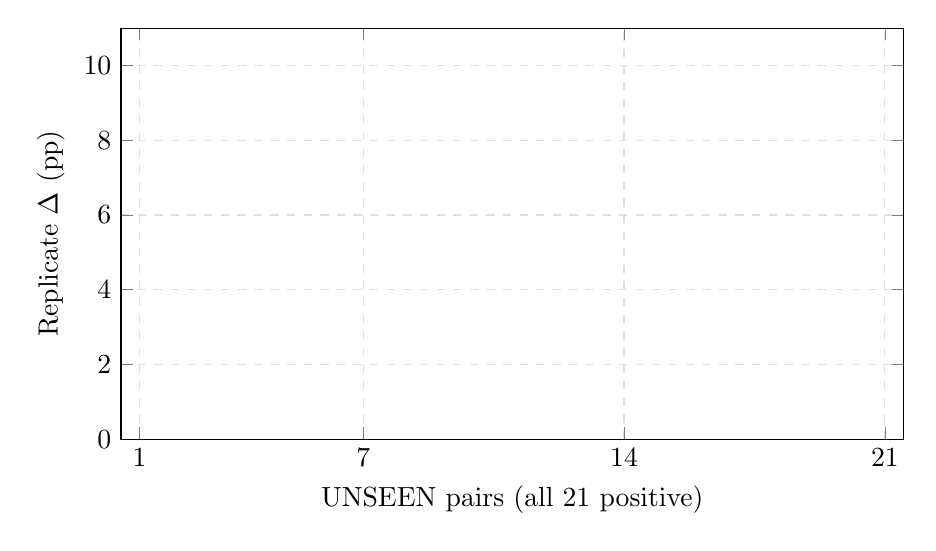
\begin{tikzpicture}
\begin{axis}[
  width=0.95\linewidth,
  height=6.8cm,
  ylabel={Replicate $\Delta$ (pp)},
  xlabel={UNSEEN pairs (all 21 positive)},
  only marks,
  mark size=2.2pt,
  ymin=0, ymax=11,
  xmin=0.5, xmax=21.5,
  xtick={1,7,14,21},
  grid=major,
  grid style={dashed,gray!25},
]
% All 21 UNSEEN replicate deltas from combined analysis (config order)
\addplot[black] coordinates {
  (1,2.12) (2,6.08) (3,8.84)
  (4,7.97) (5,3.96) (6,6.35)
  (7,7.14) (8,5.14) (9,6.96)
  (10,2.91) (11,5.00) (12,3.58)
  (13,3.67) (14,1.27) (15,5.62)
  (16,6.56) (17,7.58) (18,2.43)
  (19,6.02) (20,9.62) (21,5.70)
};
\addplot[gray,dashed,forget plot] coordinates {(0.5,0) (21.5,0)};
\end{axis}
\end{tikzpicture}
\caption{UNSEEN replicate-level paired $\Delta$ values (canonical coverage).
All 21 Direct$\leftrightarrow$Primed pairs are positive.
Points are ordered by configuration (Gemini ON, Gemini OFF, Claude, DeepSeek, Qwen, GPT-5.6 Luna, Grok), three replicates each.
Descriptive display only.}
\label{fig:replicates}
\end{figure}
